% !TEX program = xelatex
\documentclass[11pt,a4paper]{article}
\newcommand{\ZHDOC}{1}
\newcommand{\DOCFOOT}{AMPERE POINT · Q11 与 Shelly X 模组 · 测试文档 v1 · 2026 年 9 月 28 日}
% Wspólna preambuła dokumentów dla producenta (xelatex); kopia z raportu DLB, czcionki systemowe Windows
\usepackage{fontspec}
% \ZHDOC zdefiniowane przed \input => cały dokument po chińsku (Noto Sans CJK SC + łamanie wierszy CJK)
\ifdefined\ZHDOC
  \setmainfont{Microsoft YaHei}[Scale=0.90]
  \setsansfont{Microsoft YaHei}[Scale=0.90]
  \XeTeXlinebreaklocale "zh"
  \XeTeXlinebreakskip = 0pt plus 1pt minus 0.1pt
\else
  \setmainfont{Calibri}
  \setsansfont{Calibri}
\fi
\setmonofont{Consolas}[Scale=0.86]
\newfontfamily\cjkfont{Microsoft YaHei}[Scale=0.90]
\newfontfamily\latinfont{Calibri}
\newcommand{\pl}[1]{{\latinfont #1}}
\usepackage[a4paper,top=2.0cm,bottom=2.0cm,left=1.9cm,right=1.9cm]{geometry}
\usepackage{graphicx}
\usepackage[table]{xcolor}
\usepackage{booktabs,longtable,array,tabularx,enumitem,fancyhdr,caption}
\usepackage[most]{tcolorbox}
\usepackage[hidelinks,unicode]{hyperref}
\usepackage{needspace}
\usepackage{float}
\emergencystretch=2.5em
\setlength{\parindent}{0pt}\setlength{\parskip}{5pt}
\renewcommand{\arraystretch}{1.22}
\captionsetup{font=small,labelfont=bf,skip=3pt}
\setlist{nosep,leftmargin=*}
\setcounter{secnumdepth}{2}

\definecolor{apnavy}{HTML}{1A1A1A}
\definecolor{apink}{HTML}{1C2430}
\definecolor{apmuted}{HTML}{5B6675}
\definecolor{apline}{HTML}{E3E3E3}
\definecolor{apbg}{HTML}{F5F5F5}
\definecolor{apaccent}{HTML}{EC6434}
\definecolor{apaccentbg}{HTML}{FDEDE6}
\definecolor{apwarn}{HTML}{B9791B}
\definecolor{apwarnbg}{HTML}{FBF1DE}
\definecolor{apred}{HTML}{B91C1C}
\definecolor{apredbg}{HTML}{FEE2E2}
\definecolor{apgreen}{HTML}{1F8A4C}
\definecolor{apgreenbg}{HTML}{E7F5EC}
\definecolor{aphead}{HTML}{EDEDED}

\pagestyle{fancy}\fancyhf{}
\renewcommand{\headrulewidth}{0pt}
\fancyfoot[L]{\footnotesize\color{apmuted}\DOCFOOT}
\fancyfoot[R]{\footnotesize\color{apmuted}\thepage\,/\,\pageref{LastPage}}
\usepackage{lastpage}

\usepackage{titlesec}
\titleformat{\section}{\Large\bfseries\color{apnavy}}{\thesection}{0.6em}{}
\titlespacing*{\section}{0pt}{14pt}{6pt}
\titleformat{\subsection}{\large\bfseries\color{apnavy}}{\thesubsection}{0.6em}{}
\titlespacing*{\subsection}{0pt}{10pt}{4pt}

% pasek tytułowy
\newcommand{\apheader}[3]{%
\noindent
\includegraphics[height=1.0cm]{logo_ap.png}\hfill
\raisebox{0.25cm}{\parbox[t]{10.5cm}{\raggedleft\footnotesize\color{apmuted}#3}}\\[0.25cm]
{\color{apaccent}\rule{\textwidth}{1.8pt}}\\[0.30cm]
{\bfseries\color{apnavy}\LARGE #1}\\[0.18cm]
{\large\color{apmuted}#2}\\[0.2cm]}

% ramki
\newtcolorbox{apbox}[1][]{enhanced,breakable,colback=apbg,colframe=apline,boxrule=0.6pt,arc=3pt,left=7pt,right=7pt,top=5pt,bottom=5pt,fonttitle=\bfseries,coltitle=apnavy,colbacktitle=aphead,title={#1}}
\newtcolorbox{apwarnb}[1][]{enhanced,breakable,colback=apwarnbg,colframe=apwarn,boxrule=0.6pt,arc=3pt,left=7pt,right=7pt,top=5pt,bottom=5pt,fonttitle=\bfseries,title={#1}}
\newtcolorbox{apredb}[1][]{enhanced,breakable,colback=apredbg,colframe=apred,boxrule=0.6pt,arc=3pt,left=7pt,right=7pt,top=5pt,bottom=5pt,fonttitle=\bfseries,title={#1}}
\newtcolorbox{apgreenb}[1][]{enhanced,breakable,colback=apgreenbg,colframe=apgreen,boxrule=0.6pt,arc=3pt,left=7pt,right=7pt,top=5pt,bottom=5pt,fonttitle=\bfseries,title={#1}}

% komórka ze zrzutem ekranu: #1 szerokość, #2 plik, #3 podpis
\newcommand{\shot}[3]{%
\begin{minipage}[t]{#1}
  \vspace{0pt}\centering
  \includegraphics[width=\linewidth,height=6.2cm,keepaspectratio]{#2}\par\vspace{3pt}
  {\footnotesize\color{apink}#3\par}
\end{minipage}}


% mniejsza komórka ze zdjęciem (np. gniazda aut)
\newcommand{\shotsm}[3]{%
\begin{minipage}[t]{#1}
  \vspace{0pt}\centering
  \includegraphics[width=\linewidth,height=4.6cm,keepaspectratio]{#2}\par\vspace{3pt}
  {\footnotesize\color{apink}#3\par}
\end{minipage}}

\newcommand{\kroknum}[1]{{\colorbox{apaccent}{\textcolor{white}{\bfseries\small\,#1\,}}}}
\newcommand{\dpn}[1]{{\cjkfont #1}}
\newcommand{\Fact}{\textcolor{apgreen}{\textbf{[fact]}}}
\newcommand{\Hyp}{\textcolor{apwarn}{\textbf{[hypothesis]}}}

\setlength{\tabcolsep}{4pt}
\renewcommand{\figurename}{图}
\newfontfamily\symbolfont{Segoe UI Symbol}
\newcommand{\ok}{{\symbolfont\color{apgreen}\textbf{✔}}}
\newcommand{\half}{{\symbolfont\color{apwarn}\textbf{◐}}}
\newcommand{\no}{{\symbolfont\color{apred}\textbf{✘}}}
\newcommand{\ra}{{\symbolfont →}}
\newcommand{\la}{{\symbolfont ←}}
\newcommand{\hx}[1]{\texttt{#1}}
\hypersetup{pdftitle={Q11 充电桩更换 Shelly X 模组：测试文档与接口映射},pdfauthor={AMPERE POINT}}
\begin{document}

\apheader{Q11 充电桩更换 Shelly X 模组}%
{测试文档与接口映射：连接、串口协议、数据点、结果、待确认问题}%
{AMPERE POINT — 研发部 · 提供给制造商的文档\\2026 年 9 月 28 日 · 版本 1\\编写：Dawid Cekała}

{\small\color{apmuted}本文件为英文版的中文译本，内容一致；如有歧义，以英文版为准。}

\section{目的与范围}

AmperePoint 正在评估将 Q11 充电桩（贵司产品 \texttt{Q21\_11kW\_with\_OTA}，控制板 \texttt{X2Q322\_K\_V4}）中的涂鸦 WBR3 Wi-Fi 模组更换为 Shelly X 模组。本文档记录了 2026 年 9 月 24 日至 28 日在一台真实 Q11 上进行的测试：模组如何连接、控制器在串口上发送什么、其数据点如何映射、哪些测试已通过，以及哪些问题仍待确认。本文档面向贵司研发工程师。

\begin{apgreenb}[一句话结论]
Q11 控制器\textbf{无需对控制器固件做任何修改}即可与 Shelly 模组配合工作。Shelly 模组以 9600 波特率使用涂鸦 MCU 串口协议；四根连线（3.3~V、GND、RXD、TXD）即可。在 2026 年 9 月 25 日约十小时（10:51--20:48）的帧级日志中，充电开关、电流上限、工作状态、连接状态、温度、相位数据和故障位均实现了双向交换。
\end{apgreenb}

\begin{longtable}{>{\raggedright\arraybackslash}p{3.2cm}>{\raggedright\arraybackslash}p{12.9cm}}
\toprule
\rowcolor{aphead}\textbf{范围内} & \textbf{详情} \\
\midrule\endhead
\bottomrule\endfoot
硬件 & U10 模组位、主板实际使用的焊盘、控制器引脚、模组由主板供电 \\
串口链路 & 线上观察到的涂鸦 MCU 协议：启动握手、常规通信、写入行为、帧示例 \\
数据点 & 产品定义中全部 17 个数据点：类型、编码、控制器是否上报、在 Shelly 产品中如何映射 \\
测试 & 双向控制与状态、无云运行、时间下发、本地集成层（简述） \\
\rowcolor{aphead}\textbf{范围外} & \\
云与 App & 本文不描述 Shelly 云、Shelly App 界面和 AmperePoint 后台；它们对控制器没有任何要求 \\
\end{longtable}

\section{设备}

\begin{longtable}{>{\raggedright\arraybackslash}p{3.2cm}>{\raggedright\arraybackslash}p{12.9cm}}
\toprule
\rowcolor{aphead}\textbf{项目} & \textbf{详情} \\
\midrule\endhead
\bottomrule\endfoot
充电桩 & AmperePoint Q11，11~kW 三相便携式充电桩。控制板 \texttt{X2Q322\_K\_V4}（260703）。控制器：LQFP64 封装微控制器，贴有\emph{“X2Q311OW OTA V22”}标签。涂鸦 WBR3 模组已从 U10 位置拆下。 \\
原型模组 & Shelly DevKit M1 v1.1（乐鑫参考板），搭载 Shelly-X-MOD1-H8 模组（ESP32-C3 内核，Shelly 固件 \texttt{2.0.0-beta11}），见图~\ref{fig:devkit}。通过四根导线连接到 U10，并由主板供电。 \\
目标模组 & Shelly X 模组 X1，硬件版本 V020，规格书版本 14（见附件）。与 WBR3 封装相同：16~$\times$~24~mm，2~$\times$~8 焊盘，间距 2~mm。 \\
Shelly 产品配置 & 在 Shelly X 开发者门户中创建：数据源“Tuya MCU”，IO4（TX）/ IO5（RX），9600 波特，声明 7 个数据点，6 个字段（状态、电流上限、模式、相位信息、本次充电电量、本次充电时长），服务脚本 v3 由 AmperePoint 编写。 \\
工具 & 万用表（对全部 16 个焊盘做通断和二极管测试）、通过 Wi-Fi 读取的模组调试日志（帧级，每一串口帧带时间戳）、用于 MQTT 和 OCPP 测试的 Python 工具。 \\
\end{longtable}

\begin{figure}[H]
\centering
\shot{0.46\textwidth}{devkit_top.jpg}{Shelly DevKit M1 正面：USB-C、USB--UART 桥、RGB LED、带天线的 Shelly-X-MOD1-H8 模组}\hspace{0.6cm}
\shot{0.46\textwidth}{devkit_bottom.jpg}{背面：引脚标识。引脚 4 和 5（TX、RX）接到 Q11；标有 RX/TX 的引脚是 USB/日志端口，未使用}
\caption{测试所用的原型模组。}
\label{fig:devkit}
\end{figure}

\section{电气连接}

\subsection{U10 模组位：主板实际使用的焊盘}

充电桩断电，万用表二极管档，红表笔接 GND 焊盘测量。结果：\textbf{只有四个焊盘与控制器有连接}。其余焊盘对 GND、对 VCC 以及相互之间均为开路（OL）。

\begin{longtable}{>{\raggedright\arraybackslash}p{0.8cm}>{\raggedright\arraybackslash}p{1.6cm}>{\raggedright\arraybackslash}p{4.3cm}>{\raggedright\arraybackslash}p{4.3cm}>{\raggedright\arraybackslash}p{4.2cm}}
\toprule
\rowcolor{aphead}\textbf{焊盘} & \textbf{WBR3 名称} & \textbf{Q11 主板上（实测）} & \textbf{原型（DevKit）} & \textbf{目标（同位置的 Shelly X1 焊盘）} \\
\midrule\endhead
\bottomrule\endfoot
1 & NC & 无连接 & 未连接 & RESET（模组复位输入，悬空） \\
2 & A\_7 & 无连接 & 未连接 & NTC（悬空） \\
3 & EN & 无连接 & 未连接 & NC \\
4 & A\_11 & 无连接 & 未连接 & IO0 \\
5 & A\_2 & 无连接 & 未连接 & IO1 \\
6 & A\_3 & 无连接 & 未连接 & IO2 \\
7 & A\_4 & 无连接 & 未连接 & IO3 \\
8 & VCC & 主板稳压器输出 3.3~V；控制器引脚 1、13、19、32、48、64 & DevKit 的 3V3，经可拔插跳线 & 3V3 \\
9 & GND & 地；控制器引脚 12、18、31、47、63 & GND & GND \\
10 & A\_12 & 无连接 & 未连接 & Sys btn（悬空） \\
11 & A\_16 & 无连接 & 未连接 & U0TXD（维护串口，悬空） \\
12 & A\_17 & 无连接 & 未连接 & U0RXD（维护串口，悬空） \\
13 & A\_18 & 无连接 & 未连接 & IO7 \\
14 & A\_19 & 无连接 & 未连接 & IO6 \\
15 & RXD & 控制器引脚 16 = PA2，USART TX（控制器发送） & DevKit 引脚 5 = IO5，RX 输入，经 470~$\Omega$ & IO5（RX） \\
16 & TXD & 控制器引脚 17 = PA3，USART RX（控制器接收） & DevKit 引脚 4 = IO4，TX 输出，经 470~$\Omega$ & IO4（TX） \\
\end{longtable}

焊盘编号遵循 WBR3 规格书：焊盘 1 位于丝印“U10”旁的圆点处，焊盘 1--8 沿右列向上，焊盘 9--16 沿左列向下（主板从元件面观察，天线边在下方）。X1 列由 X1 规格书（IO 布局，第 5 页）与 WBR3 规格书叠加两种封装推导得出，尚未在实物 X1 样品上验证。

\begin{apbox}[这对直接替换意味着什么]
\begin{itemize}
\item X1 的电源和地落在与 WBR3 相同的焊盘上。
\item 串口链路落在 X1 的 IO4（TX）和 IO5（RX）上，与原型接线完全一致，且已验证可行。
\item X1 的 RESET、NTC、Sys btn、U0RXD 和 U0TXD 落在 Q11 主板未连接的焊盘上，因此悬空，这对 X1 是可接受的。
\item 主板未驱动 WBR3 的 EN 焊盘（模组使能）。因此控制器无法复位或关闭模组；测试期间也不需要。
\end{itemize}
\end{apbox}

\subsection{原型的连接}

U10 与 DevKit 之间四根导线（图~\ref{fig:wiring}）：VCC~\ra~跳线~\ra~3V3，GND~\ra~GND，TXD~\ra~470~$\Omega$~\ra~DevKit 引脚 4（IO4，TX），RXD~\ra~470~$\Omega$~\ra~DevKit 引脚 5（IO5，RX）。470~$\Omega$ 电阻仅用于防止接线错误（两个输出短路时：3.3~V / 470~$\Omega$ $\approx$ 7~mA）；在 9600 波特、位时间 104~$\mu$s 的条件下对信号没有影响。DevKit 完全由主板的 3.3~V 稳压器供电；插入跳线时 USB 断开。整个测试期间模组没有发生一次欠压复位，说明主板稳压器能够为包括 Wi-Fi 发射在内的 ESP32-C3 供电。

\subsection{控制器引脚}

各使用焊盘到控制器封装的通断（图~\ref{fig:mcu}）：VCC 到引脚 1、13、19、32、48、64；GND 到引脚 12、18、31、47、63；RXD 焊盘到引脚 16；TXD 焊盘到引脚 17。电源与地的分布与 LQFP64 封装的 STM32F103 / GD32F103 / GD32F303 系列一致，引脚 16/17 为 PA2/PA3，即该系列的 USART2（GD32 命名为 USART1）。具体型号被标签遮盖；见问题~1。

\begin{figure}[H]
\centering
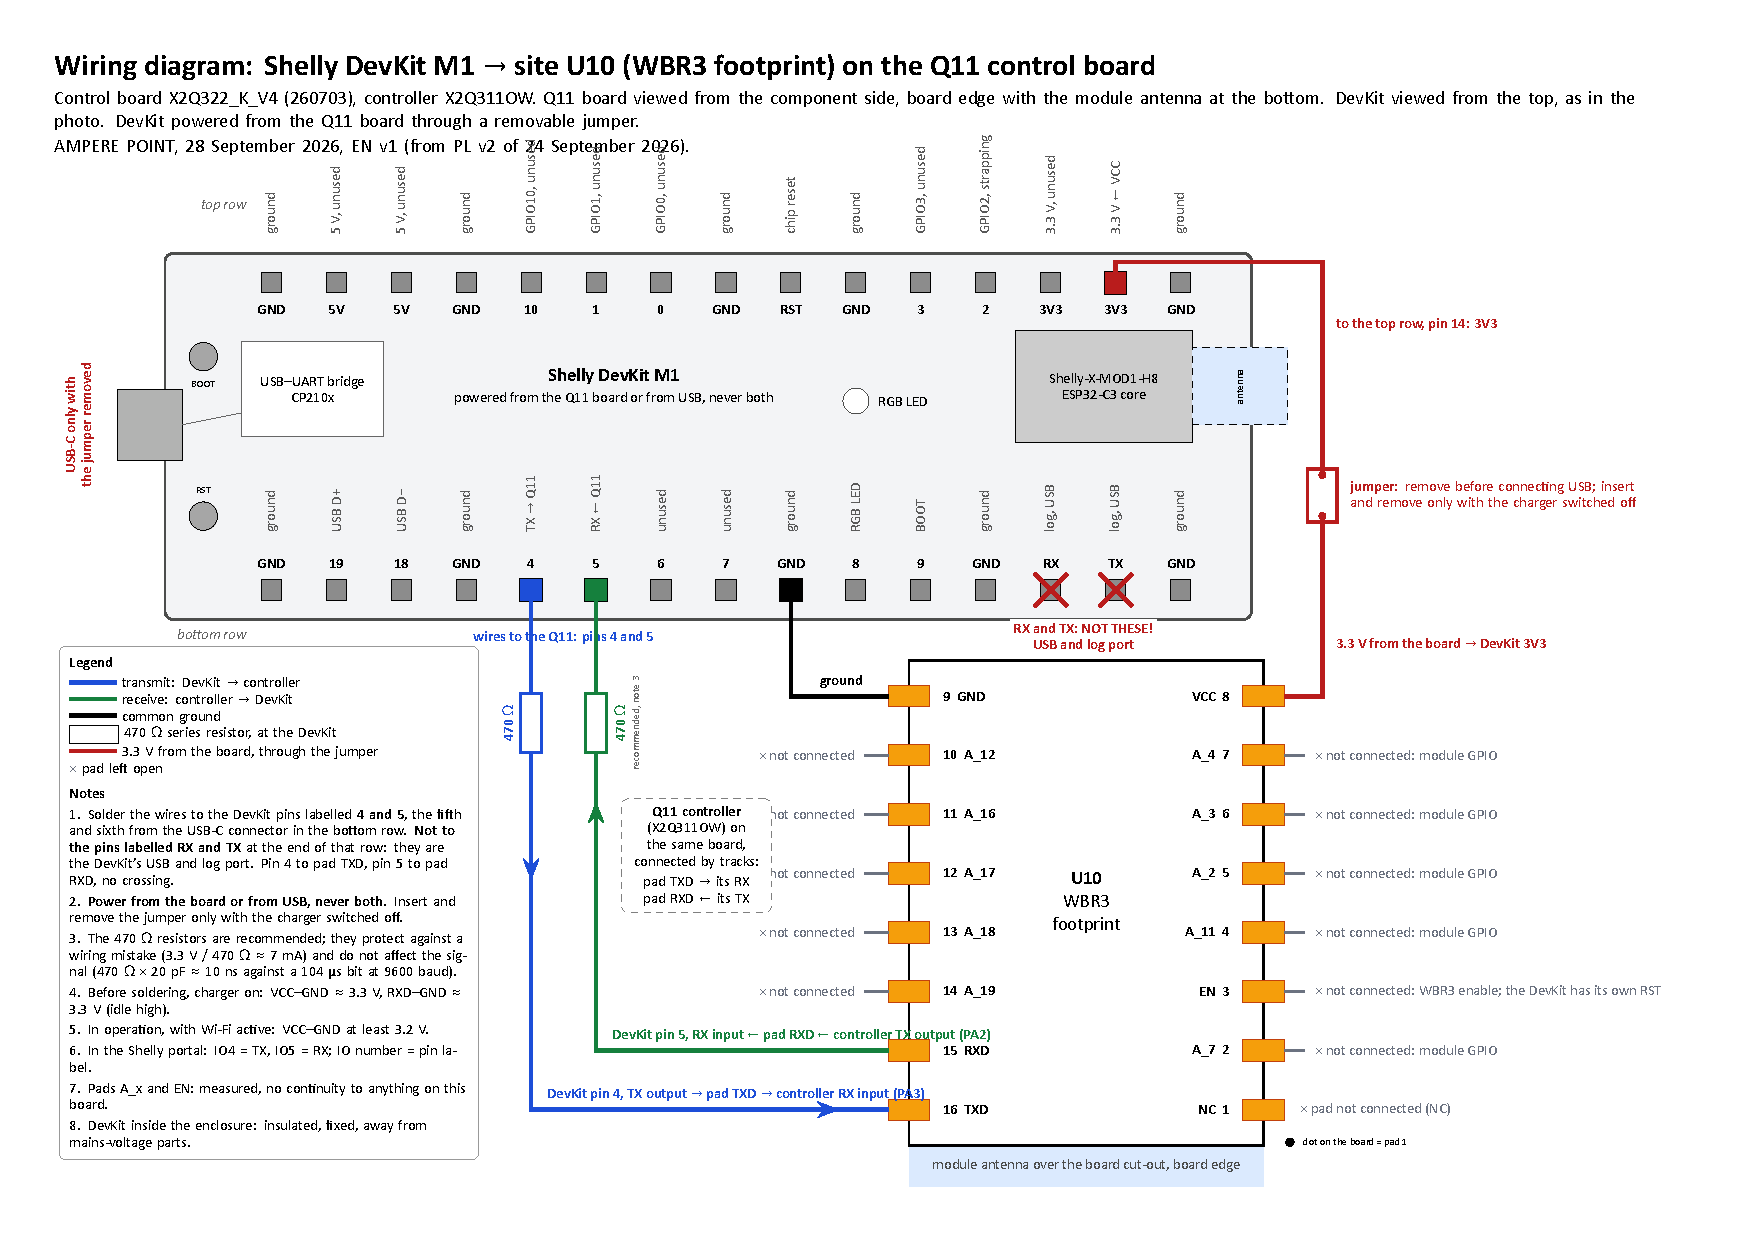
\includegraphics[width=\textwidth]{schematic_wiring_DevKit_Q11_EN.pdf}
\caption{原型接线（附完整尺寸 PDF，第 2 页显示 U10 的每个焊盘；图纸为英文）。}
\label{fig:wiring}
\end{figure}

\begin{figure}[H]
\centering
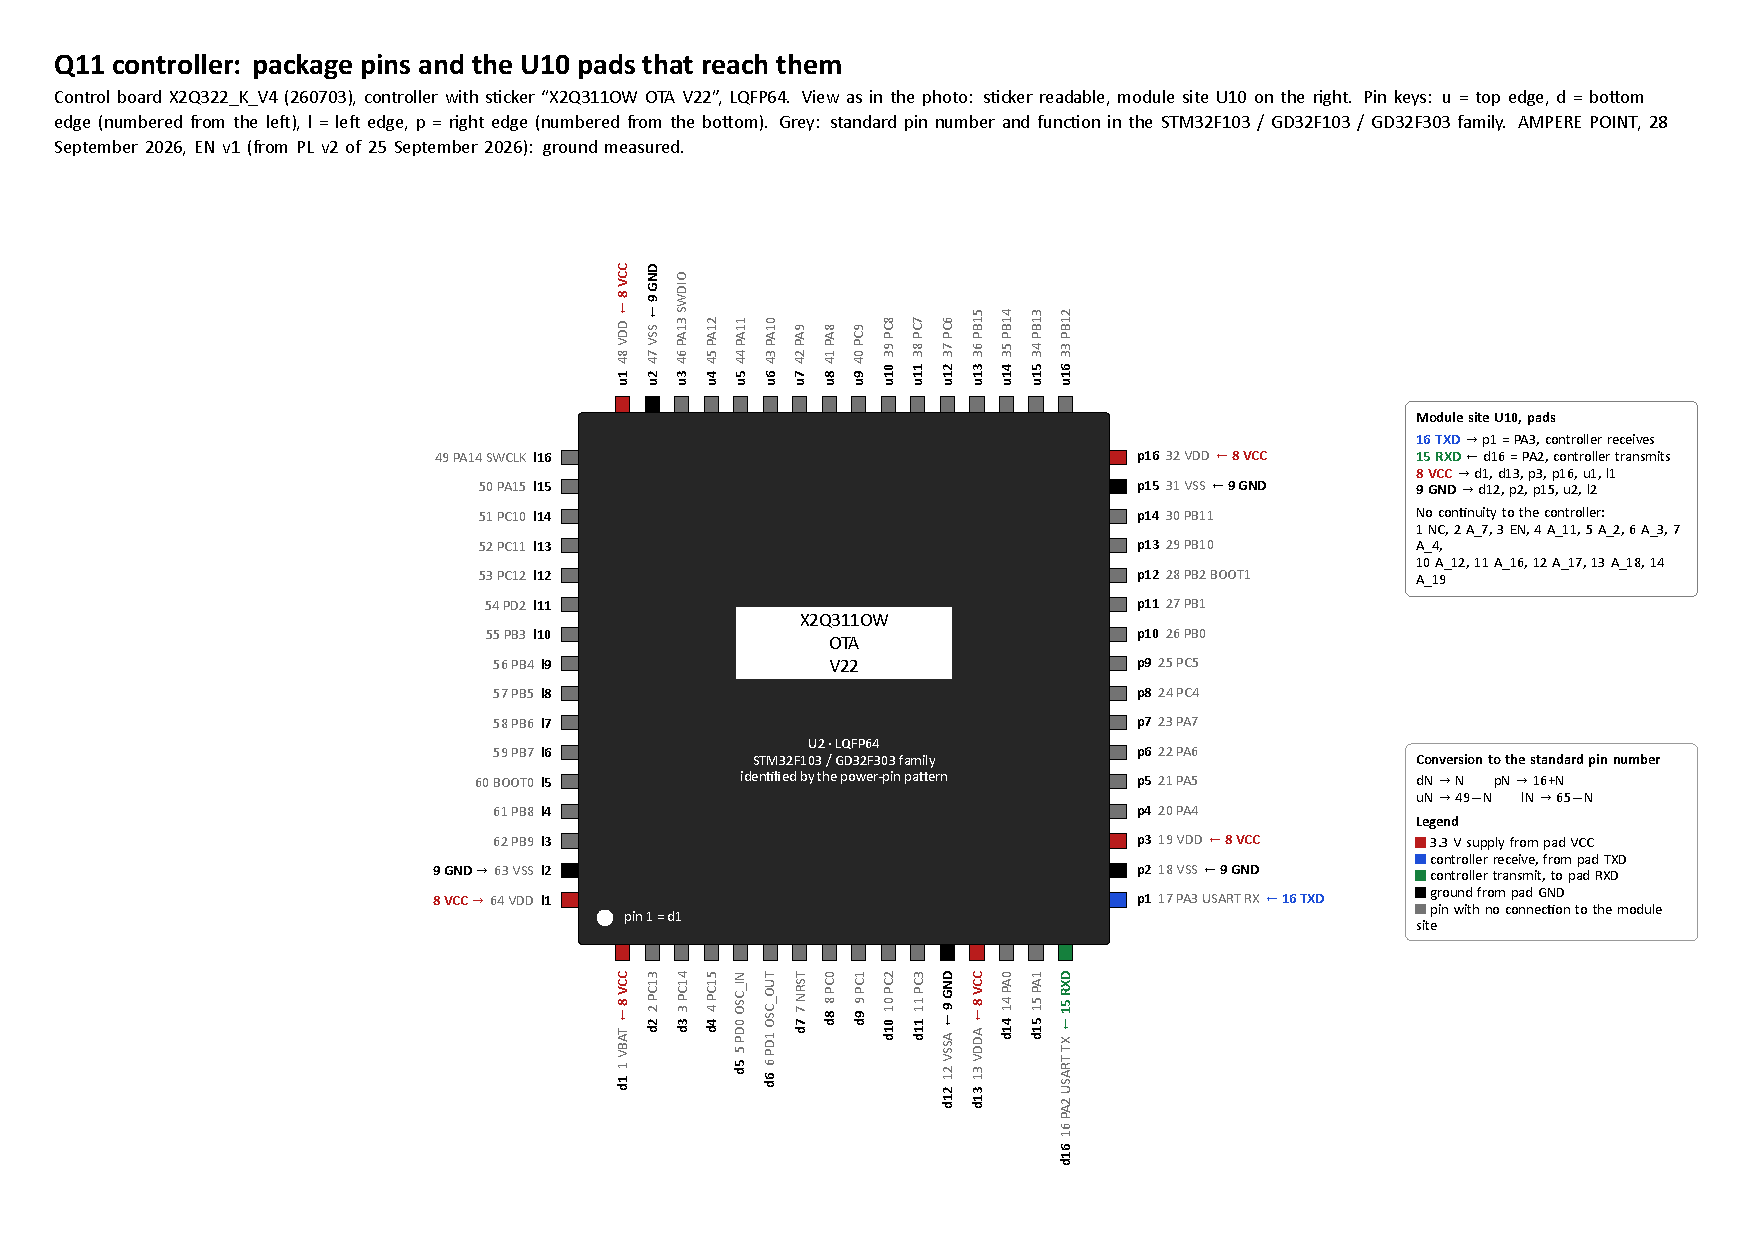
\includegraphics[width=\textwidth]{schematic_Q11_MCU_pins_EN.pdf}
\caption{控制器引脚及到达它们的 U10 焊盘（附完整尺寸 PDF；图纸为英文）。}
\label{fig:mcu}
\end{figure}

\section{线上观察到的串口协议}

\subsection{物理层与帧格式}

9600 波特，8 数据位，无校验，1 停止位，3.3~V 电平。涂鸦 MCU 串口协议：\hx{55 AA} $|$ 版本 $|$ 命令 $|$ 长度（2 字节，大端） $|$ 数据 $|$ 校验和（之前所有字节之和对 256 取模）。控制器发送版本 \hx{03}；模组发送版本 \hx{00}。Shelly 固件原生实现该协议（“Tuya MCU”组件）；AmperePoint 未编写任何协议代码。

\subsection{启动握手}

2026 年 9 月 25 日 11:51 捕获，当时模组在上传配置后重新初始化（控制器保持通电）：

\begin{longtable}{>{\raggedright\arraybackslash}p{1.6cm}>{\raggedright\arraybackslash}p{2.3cm}>{\raggedright\arraybackslash}p{4.1cm}>{\raggedright\arraybackslash}p{7.7cm}}
\toprule
\rowcolor{aphead}\textbf{时间} & \textbf{方向} & \textbf{帧（命令，数据）} & \textbf{含义} \\
\midrule\endhead
\bottomrule\endfoot
11:51:08 & 控制器 \ra\ 模组 & \hx{0x24} & 控制器请求 Wi-Fi 信号强度 \\
11:51:08 & 模组 \ra\ 控制器 & \hx{0x24 [C7]} & 应答：$-57$~dBm \\
11:51:09 & 模组 \ra\ 控制器 & \hx{0x00} & 心跳 \\
11:51:09 & 控制器 \ra\ 模组 & \hx{0x00 [01]} & 心跳应答，\hx{01} = 控制器已在运行（非刚上电） \\
11:51:14 & 模组 \ra\ 控制器 & \hx{0x03 [04]} & Wi-Fi 状态 4（涂鸦定义：已连接云） \\
11:51:14 & 控制器 \ra\ 模组 & \hx{0x03} & 已确认 \\
11:51:14 & 模组 \ra\ 控制器 & \hx{0x08} & 查询全部数据点 \\
11:51:16--17 & 控制器 \ra\ 模组 & 12 $\times$ \hx{0x07} & 数据点上报，顺序为：3、4、6、7、8、9、10、14、18、19、24、13 \\
11:51:16 & 控制器 \ra\ 模组 & \hx{0x1C} & 控制器请求时间 \\
11:51:17 & 模组 \ra\ 控制器 & \hx{0x1C [01 1A 09 19 0B 33 12 05]} & 有效，2026-09-25 11:51:18，星期 5 \\
\end{longtable}

产品信息交换（命令 \hx{0x01} 和 \hx{0x02}）发生在调试日志可通过 Wi-Fi 访问之前，未能捕获；见问题~2。

\subsection{常规通信}

\begin{itemize}
\item 模组 \ra\ 控制器：心跳 \hx{0x00} 每 15~s；Wi-Fi 状态 \hx{0x03 [04]} 每 30~s。控制器均作应答。
\item 控制器 \ra\ 模组：时间请求 \hx{0x1C} 和信号强度请求 \hx{0x24}，间隔不规则，约 10--45~s。模组只有在时钟同步（NTP）之后才应答时间请求；在此之前发送 \hx{01 00 00 00 00 00 00 00}（“有效”标志加零日期）。因此当充电桩在无互联网环境使用时，AmperePoint 提供本地 NTP 服务器。
\item 控制器 \ra\ 模组，主动 \hx{0x07} 上报：温度（DP~24）每次变化时；连接状态（DP~13）控制导引状态每次变化时；电流上限（DP~4）和开关（DP~18）每次写入后；本次充电电量（DP~25）在一次充电结束时上报一次。
\end{itemize}

\subsection{写入行为}

写入（\hx{0x06}）时，控制器先上报\textbf{旧}值，约一秒后再上报\textbf{新}值。示例，电流上限 12~A \ra\ 10~A，2026 年 9 月 25 日：

\begin{longtable}{>{\raggedright\arraybackslash}p{1.6cm}>{\raggedright\arraybackslash}p{2.5cm}>{\raggedright\arraybackslash}p{6.3cm}>{\raggedright\arraybackslash}p{5.4cm}}
\toprule
\rowcolor{aphead}\textbf{时间} & \textbf{方向} & \textbf{完整帧} & \textbf{含义} \\
\midrule\endhead
\bottomrule\endfoot
11:56:48 & 模组 \ra\ 控制器 & \hx{55 AA 00 06 00 08 04 02 00 04 00 00 00 0A 21} & 设置 DP~4（数值型，4 字节）= 10 \\
11:56:49 & 控制器 \ra\ 模组 & \hx{55 AA 03 07 00 08 04 02 00 04 00 00 00 0C 27} & 上报 DP~4 = 12（仍是旧值） \\
11:56:50 & 控制器 \ra\ 模组 & \hx{55 AA 03 07 00 08 04 02 00 04 00 00 00 0A 25} & 上报 DP~4 = 10（已接受） \\
10:52:37 & 模组 \ra\ 控制器 & \hx{55 AA 00 06 00 05 12 01 00 01 01 1F} & 设置 DP~18（布尔）= 1，允许充电 \\
10:52:38 & 控制器 \ra\ 模组 & \hx{55 AA 03 07 00 05 12 01 00 01 01 23} & 上报 DP~18 = 1 \\
-- & 控制器 \ra\ 模组 & \hx{55 AA 03 00 00 01 01 04} & 心跳应答，供参考 \\
\end{longtable}

8、10、12、14 和 16~A 的写入均以同样方式得到控制器确认。

\section{数据点}

\subsection{三个层次}

无论哪个模组在监听，控制器都在串口上发送其数据点上报；Shelly 模组接收到的每一帧与 WBR3 完全相同。不同之处在于数据点含义的定义位置：使用 WBR3 时，定义在涂鸦云的产品定义中；使用 Shelly 模组时，定义在 AmperePoint 编写的产品配置中。日志证实 Shelly 模组会登记每一个上报的数据点，包括未在产品配置中声明的数据点（日志条目如 \texttt{add int 24}、\texttt{add enum 13}、\texttt{add raw 19}）。

\begin{longtable}{>{\raggedright\arraybackslash}p{6.2cm}>{\raggedright\arraybackslash}p{3.0cm}>{\raggedright\arraybackslash}p{6.9cm}}
\toprule
\rowcolor{aphead}\textbf{层次} & \textbf{数据点} & \textbf{定义方} \\
\midrule\endhead
\bottomrule\endfoot
模组接收并保存 & 控制器发送的全部：观察到 13 个不同 ID & 控制器固件 \\
在 Shelly 产品中声明，可供服务脚本使用 & 7 个（1、3、4、6、7、8、18） & AmperePoint，在门户中 \\
作为字段暴露（App、本地 API、MQTT） & 6 个字段 & AmperePoint，在服务脚本中 \\
\end{longtable}

枚举在线上以索引字节传输；名称仅存在于产品定义中。Shelly 产品使用与涂鸦定义相同的顺序（问题~7 请求确认）。

\subsection{对比：涂鸦产品定义、控制器行为、Shelly 产品}

定义取自涂鸦产品 \emph{Ampere Point Q11 PRO}（17 个数据点）。“上报” = 2026 年 9 月 25 日模组日志中观察到：\textbf{汇总} = 在对查询 \hx{0x08} 的应答中，\textbf{主动} = 控制器自行发送，\textbf{从未} = 任何帧中均未出现。

\begin{longtable}{>{\raggedright\arraybackslash}p{0.7cm}>{\raggedright\arraybackslash}p{3.1cm}>{\raggedright\arraybackslash}p{3.6cm}>{\raggedright\arraybackslash}p{0.9cm}>{\raggedright\arraybackslash}p{3.2cm}>{\raggedright\arraybackslash}p{3.8cm}}
\toprule
\rowcolor{aphead}\textbf{DP} & \textbf{涂鸦代码} & \textbf{类型、单位、编码} & \textbf{读写} & \textbf{控制器上报} & \textbf{在 Shelly 产品中} \\
\midrule\endhead
\bottomrule\endfoot
1 & forward\_\allowbreak energy\_\allowbreak total & 数值，kWh，比例 2（\hx{123456} = 1234.56~kWh） & R & \no\ 从未（不在汇总中，也不主动） & 已声明，用于累计电量；因无数据而保持为 0。问题~4 \\
3 & work\_state & 枚举，8 种状态：0 free，1 insert，2 free\_fault，3 wait，4 charging，5 pause，6 end，7 fault & R & \ok\ 汇总；观察到值 0 和 3 & \ok\ 字段“mode”，索引翻译为名称 \\
4 & charge\_cur\_set & 数值，A，6--32 & RW & \ok\ 汇总；写入 8/10/12/14/16 均确认 & \ok\ 字段“current limit”，针对 Q11 限制为 6--16~A \\
6、7、8 & phase\_a / b / c & 原始，7 字节：电压 2 字节 $\times$0.1~V，电流 3 字节 $\times$0.001~A，功率 2 字节，单位 W & R & \ok\ 汇总；接触器闭合时观察到 226--228~V；带载时的电流和功率尚未观察 & \ok\ 在脚本中解码为“phase info”字段 \\
9 & power\_total & 数值，kW，比例 3 & R & \ok\ 汇总；0 & \half\ 脚本改为对各相求和 \\
10 & fault & 位图，17 位：ov\_cr, ov2\_cr\_fault, ov\_vol, undervoltage\_alarm, contactor\_adhesion, contactor\_fault, earth\_fault, meter\_hardware\_alarm, scram\_fault, cp\_fault, meter\_commu\_fault, card\_reader\_fault, cir\_short\_fault, adhesion\_fault, self\_test\_alarm, leakagecurr\_alarm, ov\_Temp\_fault & R & \ok\ 汇总；0 & \half\ 已接收，尚未作为字段暴露 \\
13 & connection\_state & 枚举，7 种：0 12V，1 12V\_pwm，2 9V，3 9V\_pwm，4 6V，5 6V\_pwm，6 error & R & \ok\ 汇总 + 主动；观察到值 0、2、4 & \half\ 已接收，尚未暴露 \\
14 & work\_mode & 枚举，3 种：0 charge\_now，1 charge\_energy，2 charge\_schedule & RW & \ok\ 汇总；0 & \half\ 已接收，尚未暴露 \\
17 & energy\_charge & 数值，kWh，1--200 & RW & \no\ 从未 & 未声明。问题~4 \\
18 & switch & 布尔 & RW & \ok\ 汇总 + 写入后主动 & \ok\ 字段“state” \\
19 & local\_timer & 原始，2 字节：起始小时、结束小时 & RW & \ok\ 汇总；\hx{00 00} & \half\ 已接收，尚未暴露 \\
23 & system\_version & 字符串 & R & \no\ 从未 & 未声明。问题~4 \\
24 & temp\_current & 数值，°C，$-40$--200 & R & \ok\ 汇总 + 变化时主动；18--20~°C & \half\ 已接收，尚未暴露 \\
25 & charge\_\allowbreak energy\_\allowbreak once & 数值，kWh，比例 2 & R & \half\ 一次：值 0，与 DP~18 = 0 在同一帧中 & \half\ 本次充电电量目前在脚本中计算；将改用 DP~25 \\
33 & mode\_set & 原始 & RW & \no\ 从未 & 未声明。问题~5 \\
\end{longtable}

对 \hx{0x08} 的应答汇总包含 12 个数据点，顺序为：3、4、6、7、8、9、10、14、18、19、24、13。数据点 1、17、23 和 33 不在汇总中，也从未单独发送。

\section{测试结果}

\begin{longtable}{>{\raggedright\arraybackslash}p{4.2cm}>{\raggedright\arraybackslash}p{1.7cm}>{\raggedright\arraybackslash}p{10.1cm}}
\toprule
\rowcolor{aphead}\textbf{测试} & \textbf{结果} & \textbf{详情} \\
\midrule\endhead
\bottomrule\endfoot
与控制器通信 & \ok & 涂鸦 MCU 协议，9600 8N1；心跳有应答；数据点有上报；控制器固件未作修改 \\
主板使用的焊盘 & \ok & 仅 VCC、GND、RXD、TXD；十二个焊盘开路 \\
模组由主板供电 & \ok & 主板稳压器 3.3~V；测试期间无欠压 \\
从模组控制充电开关 & \ok & 写入 DP~18，控制器在 1~s 内确认 \\
从模组设置电流上限 & \ok & 写入 8、10、12、14、16~A 并确认 \\
状态读取 & \ok & 工作状态、连接状态、温度、故障位、工作模式、定时窗口、相电压 \\
向控制器下发时间 & \ok & 模组获得 NTP 后以正确本地时间应答 \hx{0x1C}；离线时使用本地 NTP 服务器 \\
向控制器发送 Wi-Fi 状态 & \ok & 每 30~s 发送 \hx{0x03 [04]}；充电桩显示屏显示网络图标 \\
完全无云运行 & \ok & 关闭 Shelly 云；通过本地网络（HTTP、WebSocket、MQTT）和蓝牙控制模组 \\
本地集成层 & \ok & 见下文 \\
带载充电 & \half & 使用车辆模拟器测试了控制导引状态；带电流的完整充电尚待进行 \\
通过模组更新控制器固件 & \no\ 未测试 & 见问题~9 \\
从充电桩菜单复位 Wi-Fi & \no\ 未测试 & 见问题~8 \\
\end{longtable}

\begin{apbox}[本地集成层（中间件），供参考]
Shelly 模组提供本地 API（HTTP、WebSocket、MQTT）。在此之上，AmperePoint 在充电桩之外运行一个小型软件层：MQTT 代理、本地 NTP 服务器，以及一个将 Q11 以 OCPP~1.6J 充电点身份呈现给充电后台的桥接程序（注册、状态、远程启动、通过充电配置文件设置电流上限、电表数据）。所有这些均已用本地测试服务器验证。它运行在电脑或服务器上，而不在充电桩内，\textbf{对控制器固件没有任何要求}。在此提及只是为了呈现完整的全貌。
\end{apbox}

\section{请贵司确认的问题}

\begin{enumerate}
\item \textbf{控制器型号。}“X2Q311OW OTA V22”标签下是哪款微控制器（STM32F103xx、GD32F103xx、GD32F303xx 或其他）？Flash 容量是多少？
\item \textbf{产品信息帧。}控制器对产品查询（\hx{0x01}）的应答内容是什么：产品 key \texttt{p}、固件版本 \texttt{v}、模组工作模式 \texttt{m}？固件实现的是哪个涂鸦 MCU SDK / 协议版本？由于该交换发生在模组日志可访问之前，我们未能捕获。
\item \textbf{未连接的焊盘。}U10 的十二个焊盘（NC、A\_7、EN、A\_11、A\_2、A\_3、A\_4、A\_12、A\_16、A\_17、A\_18、A\_19）与任何位置均无通断。请根据原理图确认主板仅使用模组的 VCC、GND、RXD 和 TXD，且固件不期望其他焊盘上有任何信号（例如 EN 或复位线）。
\item \textbf{从未上报的数据点。}DP~1（forward\_energy\_total）、DP~17（energy\_charge）、DP~23（system\_version）和 DP~33（mode\_set）不在汇总中，也从未单独发送。控制器在什么条件下上报它们？DP~25（charge\_energy\_once）曾与 DP~18 = 0 一起发送过一次，值为 0：这是否是充电结束时的上报？
\item \textbf{DP~33 mode\_set。}该原始数据点的字节格式和含义是什么？
\item \textbf{DP~8。}在 \texttt{Q21\_11kW\_with\_OTA} 的导出中 DP~8 名为 \texttt{charger\_events}，在 \emph{Q11 PRO} 定义中名为 \texttt{phase\_c}。我们的样机将 DP~8 作为 7 字节原始值发送，格式与 DP~6 和 DP~7 相同。出厂固件遵循哪个定义？不同固件版本之间格式是否不同？
\item \textbf{枚举顺序。}请确认上表中 DP~3、DP~13 和 DP~14 的索引顺序。
\item \textbf{Wi-Fi 状态与配网。}控制器使用哪些 Wi-Fi 状态值（\hx{0x03}，0--7），用途是什么（显示图标、行为）？充电桩菜单中的网络复位/配网项向模组发送什么（\hx{0x04} 还是 \hx{0x05}）？
\item \textbf{通过模组更新控制器固件。}控制器是否支持涂鸦 MCU 升级命令（\hx{0x0A} 开始，\hx{0x0B} 传输数据包）？上传到涂鸦平台用于 MCU OTA 的文件是什么格式（纯二进制？），能否将同一文件提供给 AmperePoint，以便实现了相同升级命令的 Shelly 模组更新控制器？Bootloader 是否能承受升级中断？
\item \textbf{时间。}控制器每 10--45~s 请求一次时间（\hx{0x1C}）。它将时间用于什么（定时窗口 DP~19、显示、充电记录）？如果模组一直不提供有效时间会怎样？
\item \textbf{模组静默时的行为。}当模组一整天没有发送任何数据时（原型接线错误），控制器仍正常工作。心跳或 Wi-Fi 状态是否有任何超时会改变控制器的行为？
\end{enumerate}

\section{附件}

\begin{itemize}
\item \texttt{ShellyX\_module\_X1\_datasheet\_v14.pdf}：目标模组规格书（Shelly）。
\item \texttt{schematic\_wiring\_DevKit\_Q11\_EN.pdf}：原型接线及 U10 每个焊盘的功能（英文）。
\item \texttt{schematic\_Q11\_MCU\_pins\_EN.pdf}：控制器引脚及到达它们的 U10 焊盘（英文）。
\item 模组帧级日志（2026 年 9 月 25 日）可应要求提供。
\end{itemize}

{\color{apmuted}\small AMPERE POINT — 研发部 · www.amperepoint.pl · 2026 年 9 月 28 日，依据对一台 Q11 样机的测量、模组调试日志和涂鸦产品定义编写。}

\end{document}
